%%%%%%%%%%%%%%%%%%%%%%%%%%%%%%%%%%%%%%%%%%%%%%%%%%%%%%%%
%%%%%%%%%%%%%%%%%%%%%%%%%%%%%%%%%%%%%%%%%%%%%%%%%%%%%%%%
\section{Discussion}
\label{sec:discussion}
%%%%%%%%%%%%%%%%%%%%%%%%%%%%%%%%%%%%%%%%%%%%%%%%%%%%%%%%
%%%%%%%%%%%%%%%%%%%%%%%%%%%%%%%%%%%%%%%%%%%%%%%%%%%%%%%%
%
Overall, the main observation of this study was how FIM performance can be improved by reducing the Horton-Strahler stream order of the target stream network used for HAND computation.
Most of this change is accounted for by substantially increasing POD and inundation extents in some areas thus reducing FNs.
We believe, as we later argue, that the increase in POD is primarily driven by an increase in the catchment sizes that is inherently enabled by dividing up the stream network into independent stream networks of unit stream order.
Additionally, we note that reducing drainage order also has some minor influence on reducing inundation extents in other areas and the rate of false alarms.
We believe that this effect is driven by a change in the stage-discharge relationship where a given streamflow leads to lower river stage values when HAND is computed with target stream networks of unit drainage order.
We seek to explain that these two effects, catchment boundary enlargement and stage-discharge curve lowering, are highly interrelated and cannot be easily detangled.
Lastly, we discuss the diminishing effects on performance that the MS and GMS techniques may have and also any additional effects including enhanced cross-walking abilities.

As evident in the results of the study in Section \ref{sec:results}, a sizable amount of the increase in CSI observed by reducing stream order for HAND computation can be attributed to increases in POD.
This can be inferred by close inspection of Figure \ref{fig:violin_plot} and Table \ref{tab:aggregate_metrics} where changes in POD are significantly higher than that of FAR.
This intuition is confirmed by previously mentioned work by \citeA{gerapetritis2004behavior} where CSI was shown to be a direct function of both POD and FAR where CSI is maximized when $POD = 1 - FAR$.
Upon investigation of the performance of HAND derived FIM, we note a general increase of catchment sizes for the MS and GMS methods when compared to the FR method as they are now delineated independently of any tributaries that would constrain catchment sizes otherwise.
Additionally, we note significantly less water build up along catchment boundaries especially at the junction of lower order tributaries with lower flow rates and higher order rivers with more flow.
This allows for inundation extents to expand across regions previously encapsulated by catchments of joining reaches in lower flow tributaries.
The water built up along the catchment boundaries can be thought of as a column of water in a cylindrical container (catchment) that has exceeded the elevation of the container's rim which does not represent accurate physics.

Large scale HUC8 level evaluations can fail to demonstrate fine grain enhancements as they aggregate away many changes that are only clear at more local scales.
Future assessments of OWP FIM should consider finer grain evaluation units as well possible impact assessments using asset information such as building footprints to better illustrate fine grain changes in a more relevant manner to stakeholders.
For now, we provide Figure \ref{fig:gms_enhancement} which best illustrates the improvement offered by multi-source fluvial flooding capabilities in a more local context.
The figure is comprised of two agreement rasters for two different HAND based FIMs compared to the validation dataset for a given region with a high flow mainstem (500 yr recurrence flow) running horizontally along the region.
Sub-figure \ref{fig:gms_enhancement}a demonstrates the agreement raster for the FR stream network as well as its respective catchment boundary lines symbolized in white and stream network shown in green.
Inspection of this sub-figure denotes a clear spatial pattern where TPs or areas correctly inundated are pooled alongside catchment boundary lines. 
On the other side of the catchment boundary, one can witness large swaths of FNs that should be inundated. 
The FNs also exhibit a spatial pattern as in they tend to collocate within catchments of the pictured mainstems tributaries.
This sort of behavior was introduced early in the paper and shown qualitatively in Figure \ref{fig:catchment_boundaries_issue}.

As an enhancement, this paper proposes computing HAND for stream networks comprised of level-paths independently of one another.
In sub-figure \ref{fig:gms_enhancement}b, the agreement raster for the GMS technique is illustrated as well as the stream network lines in green.
While the entire mosaiced inundation map from GMS (as described in Section \ref{ssec:inundation_mapping} and Equation \ref{eq:hand_fim_depth}) is used to produce this agreement map, we only show the catchments associated with the mainstem of this region that is shown to follow a clear horizontal path.
Showing all the catchments for the tributaries that were all derived independently would convolute the image.
The main message illustrated here is that the catchments associated with the mainstem of this area significantly increase in size.
Since they are not restricted by the catchments of tributaries that lie in the same drainage areas as those of the mainstem, they extend to include those as well.
The consequence for inundation extents is a general increase in spatial coverage of the river's water which shows to be in much better agreement with the benchmark map.
The TPs are no longer bounded by the catchment lines and allowed to expand to their natural extents.
Additionally, this study has a limitation in that it did not assess FIM depths, so limited conclusions can be made about the impact of drainage order reduction techniques on the accuracy of FIM depths or water surface elevations.

We note here as a contribution of this study that a major inherent, limitation of HAND is the ``nearest drainage'' constraint or the idea that a given river reach only drains or, in HAND's case, inundates its immediate, unique drainage area or catchment.
In other words, HAND based FIMs are limited to producing fluvial inundation to only their nearest drainage area or catchment.
However, we know that fluvial inundation can be sourced from several streams nearby that also serve as drainage outlets to the area in question.
Generally speaking, drainage areas are known to be hierarchical in nature so a given drainage area for a given outlet point can be decomposed into nested drainage areas for outlet points that lie in the original drainage area.
A perfect example of this are points that lie on tributary reaches closely neighboring a mainstem.
These points lie in the drainage area of reaches in the mainstem but inundation from the mainstem cannot reach these tributary catchments because of the ``nearest'' assumption in HAND.
Hence it's important to state that just like there are different sources of flooding such as fluvial, pluvial, groundwater, reservoir, barrier failure (dam/levee/embankment), and coastal, there can also be multiple sources of a riverine flood.
HAND is only equipped to handle riverine flooding from the nearest drainage line.
Other relevant drainage lines that produce fluvial flood waters are not considered here especially if the routing model used doesn't consider backwater effects.

The remaining portion of the improvement in CSI was found to come from a marginal yet notable reduction in FAR.
Upon investigation of the spatial results in the agreement maps, we found some areas of slight reductions in FPs especially where changes in catchment boundaries may have occurred due to the reduction in effective stream order in computing HAND.
These observations pointed to changes in the SRCs introduced by stream order reduction and catchment definition adjustments.
Figure \ref{fig:rating_curve_comparison} illustrates the general effect that stream order reduction has on SRCs.
Sub-figure \ref{fig:rating_curve_comparison}a shows how the average SRCs for all reaches for stage values 0 to 25 meters at one-third meter intervals tend to shift the curve down and to the right with ever increasing stream order reduction (FR to MS to GMS). 
This bias is more pronounced for GMS since that implements stream order reduction down to the unit level for the entire FR network while MS only does so for 4-5\% of the network.

Attempting to diagnose this bias in the SRC leads one to Equation \ref{eq:reach_averaged_mannings_equation} which shows the reach averaged SRC relationship between stage and discharge.
Across the three methods explored, FR, MS, and GMS, one identifies differences in the inputs and outputs and notes no difference in the stages and Manning's n values.
While the channel slope and reach lengths are not exactly the same across methods, their averaged differences were found to be statistically insignificant which only leaves room for deviations in volume and bed area.
Specifically, we found FR to have an average reach length for the study region of 1354.8 km with a standard deviation 249.6km.
For GMS, we computed an average reach length of 1398.1 km with a standard deviation of 50.2 km.
Again, volume (V(y) or simply V) is synonymous to reach-averaged cross-sectional area and bed area (B(y) or B) is analogous to reach-averaged hydraulic radius but these associations only hold when reach length, L, is considered.
Discharge, Q, is directly related to volume and inversely related to bed area and each parameter is weighed according to the magnitude of its exponent which are $\frac{5}{3}$ and $\frac{2}{3}$ respectively (see Equation \ref{eq:reach_averaged_mannings_equation}). 
Figures \ref{fig:rating_curve_comparison}b and \ref{fig:rating_curve_comparison}c show how volume and bed area compare across the three methods with GMS having significantly greater values than MS which has greater values than FR.
Again the relative discrepancy between FR vs MS and MS vs GMS is explained by the extent of their spatial coverages.
Both V and B values increase but are weighed differently by their respective exponents and pull Q in different directions.
We show in Figure \ref{fig:rating_curve_comparison}d the relationship of $\frac{V^{5/3}}{B^{2/3}}$ and plot this ratio against stage, y, to show how these two parameters collectively pull the Q up and changes the SRC accordingly.
In other words, the magnitude and weight of the volume at each stage level exceeds the influence of the magnitude and weight of the bed area.
Both parameters are set to increase mainly due to much larger catchments leading to more pixels at each stage level as shown in Figure \ref{fig:rating_curve_comparison}e.

Much of the increase in inundated pixels, volume, and bed area can be explained by much larger catchments that encompass neighboring tributaries.
These tributaries have a significant amount of bathymetry that is low-lying thus easily included in the geometry for the SRC derivation. 
They also contribute volume and bed area that is technically not perpendicular to the flux of streamflow being accounted for in the stream in question. 
Careful examination of Figure \ref{fig:gms_enhancement}b shows how much larger catchments include neighboring tributaries and the geometry associated with those tributaries. 
This geometry is not perpendicular to the flow that is associated with the main reach thus leading to biases in the SRC.
We consider this to have a nuanced effect on skill, while reducing the rate of FPs it also can lead to FNs due to biases in the SRC.

We note that reducing stream order does suffer from diminishing returns where the increase in mapping skill for applying stream order reduction to roughly 4-5\% of the stream network is about the same as the increase for applying stream order reduction to the remaining 95-96\% of the stream network.
This motivates further work in identifying what the optimal coverage of stream order reduction could be and how to parameterize that coverage. 
One option could be removing lower stream orders (e.g. 1 and 2) from stream order reduction and simply using the inundation from FR from these areas.

Additional analysis of Figure \ref{fig:gms_enhancement}a, reveals that some catchments don't have inundation or significant inundation.
While the cause of these errors can be varied, we assert here that conflating four networks for use in evaluations leads to significant error.
Section \ref{sssec:cross_walking_networks} details how reach identifiers are conflated for the FIM network back to that of the NWM. 
One of the issues with the FR version of HAND occurs when a reach of given stream order accidentally conflates to that of a neighboring tributary that is of lower order which leads to areas of FNs.
The utilization of MS and GMS only conflates to NWM catchments directly associated with the LP in question which is inherently easy to do with those methods. 
Thus part of the improvement in MS and GMS methods is due to a slight improvement in cross-walking methodology.
The NWM stream network was derived using the NHDPlus V2 dataset which was derived from coarser DEMs than those used here. 
Additional conflation errors are realized by cross-walking the stream network used by the BLE maps and those of HAND.
The methods that intersect HEC-RAS cross-sections with NWM reaches could introduce errors that violate mass conservation.
Additionally, as previously noted and illustrated in Figure \ref{fig:ble_evaluation_method}, the BLE network is denser than that of the NWM which leads to FNs due to headwater streams that are present in the BLE but not within the NWM.
Until a singular stream network is used for the NWM, BLE benchmark, and for HAND based FIM, conflation will continue being a source of error.

Our qualitative analysis suggests that the SRCs offer a significant opportunity for improvement in HAND based FIM for future development.
The bathymetry of the 10 m DEM from 3DEP is known to be lacking proper representation thus leading to inadequate representation of volume and bed area with all three methods employed.
Manning's n which typically accounts for roughness could be tuned to account for these DEM limitations or could be held fixed to some local value associated with a given flood magnitude.
Some adjusting parameter must be introduced to enhance the estimation of the bathymetric representation.
Lidar DEMs from the USGS at 3 m and 1 m scale could be utilized to derive HAND as well which we conject should show better agreement with higher fidelity FIMs also derived from the same Lidar based DEMs.
We suspect that a significant amount of the difference in performance between 100 yr and 500 yr magnitude events can be attributed to poor SRC performance due to poor bathymetric representation.
Lower magnitude events are, logically, more susceptible to poor bathymetric data due a greater proportion of the inundation being attributable to areas that are more typically under normal flow conditions.
Higher flow events tend to cover regions with more floodplain inundation thus less sensitive to errors from bathymetric data quality.
On a related note, the use of the AGREE DEM method discussed in Section \ref{ssec:stream_network_enforcement} and \ref{sec:app_stream_network_enforcement} also interacts with the bathymetry issue introducing several artificial geometry parameters that affect SRC shape and quality.
To reiterate in this discussion, Section \ref{ssec:evaluation} pointed out that the BLE's representation of reservoir inundation extends beyond the NWM's defined reservoir boundaries, which results in an under-prediction in the OWP FIM that is reflected in the computed metrics.
Due to focus on the nearest drainage problem, we leave future work related to SRC representation including roughness estimation, bathymetric data assimilation and adjustments as well as reservoir inundation as opportunities for major enhancements in HAND based FIM.

Lastly, after errors introduced by conflation, poor roughness estimation, bathymetric/elevation adjustment, and reservoir representation are accounted for, HAND still has another fundamental limitation that is inherently baked into how it works.
For HAND to be derived and thus create a FIM for a given area, that area must entirely drain to the stream network and the stream network must also drain itself.
In other words, an entire area eligible for flooding must monotonically decrease in elevation. 
DEM's naturally don't do this and the dynamics of true flood events don't follow drainage patterns.
Enforcing this assumption for HAND leads to significant amount of DEM manipulations that introduce basic errors.
These errors are deep into the assumptions of HAND and thus more difficult to disentangle.
Ultimately, the use of more advanced 2D hydrodynamic models should be considered for dealing with this limitation of HAND but would come at significant expense at the given high resolution across very large spatial scales and frequent forecast resolutions.
%
\begin{figure}[H]
\centering
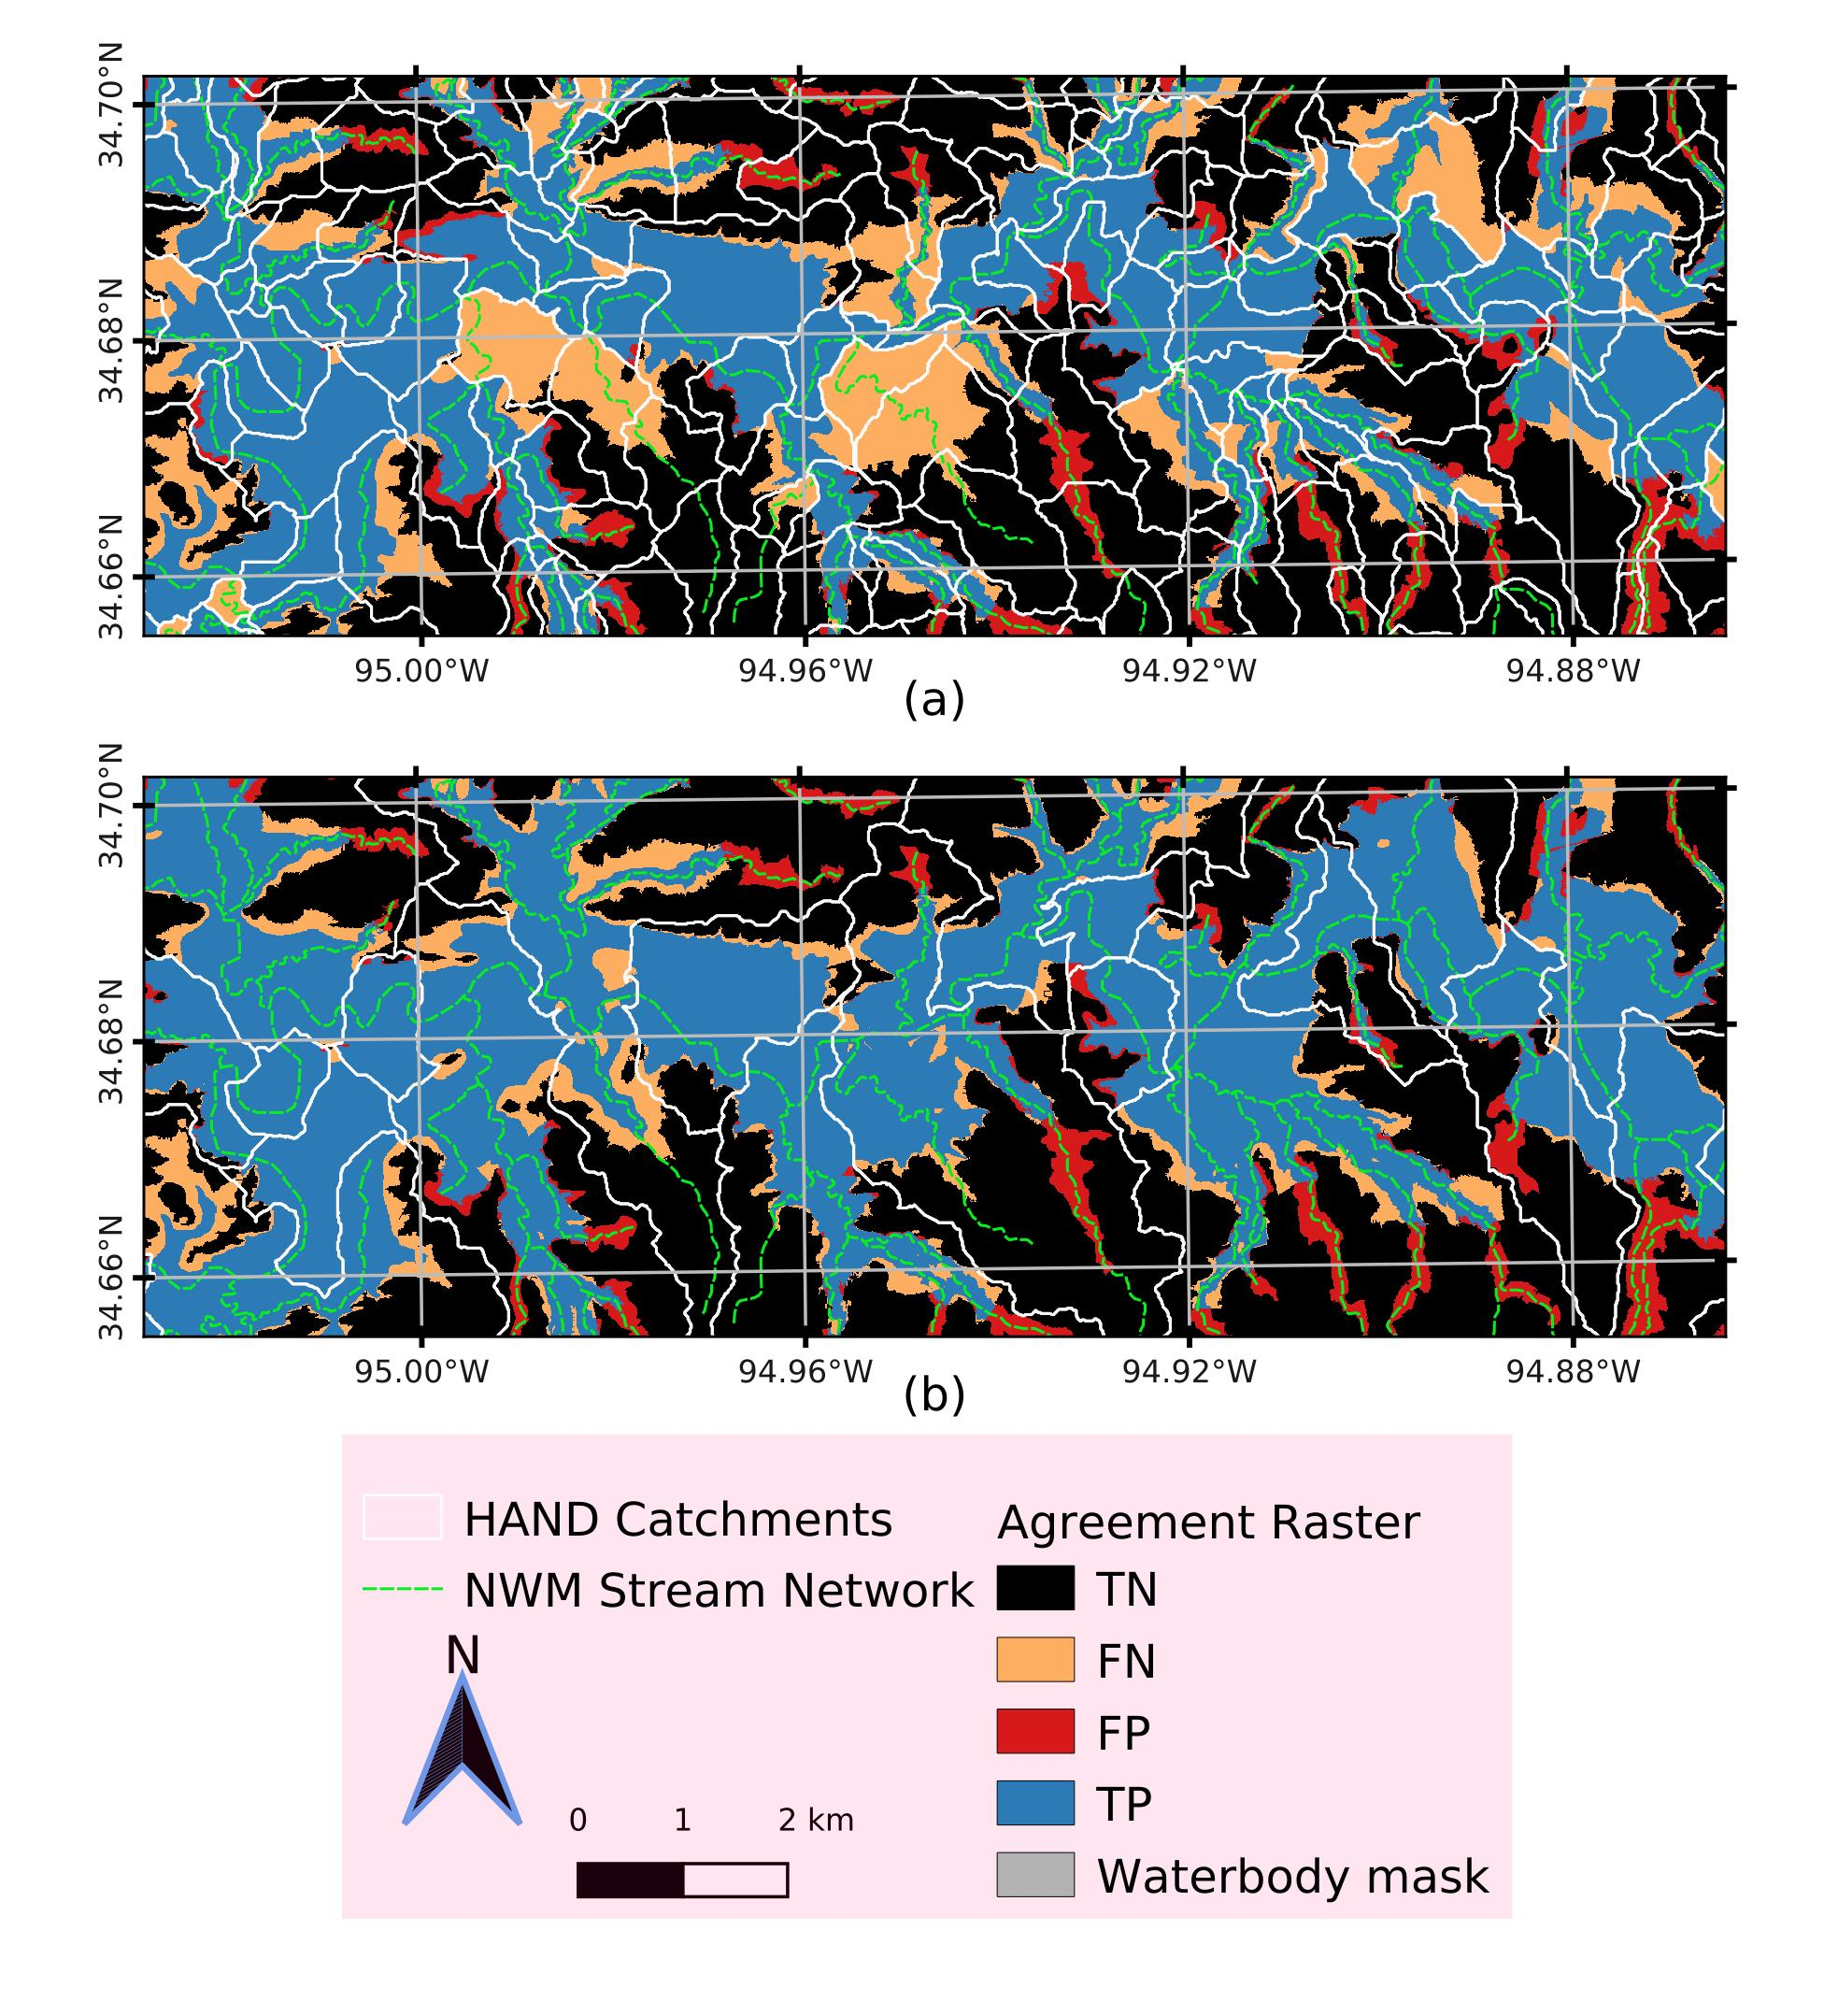
\includegraphics[scale=1.0]{figures/gms_enhancement.jpg}
\caption{OWP FIM inundation agreement, TP, FP, FN, and TN, with BLE HEC-RAS maps in HUC 11140105 at the 500 yr recurrence magnitude.
Catchment boundaries and stream lines are shown in white and dotted green, respectively.
Sub-figure (a) shows agreement of FR HAND denoting significant areas of under-prediction due to junctions and catchment boundaries.
Meanwhile, (b) shows the agreement for GMS and much larger catchments leading to much better inundation agreement for this given reach. 
Overall, this illustrates the benefits of stream order reduction for deriving HAND datasets.
}
\label{fig:gms_enhancement}
\end{figure}
%
%
\begin{figure}[H]
    \centering
    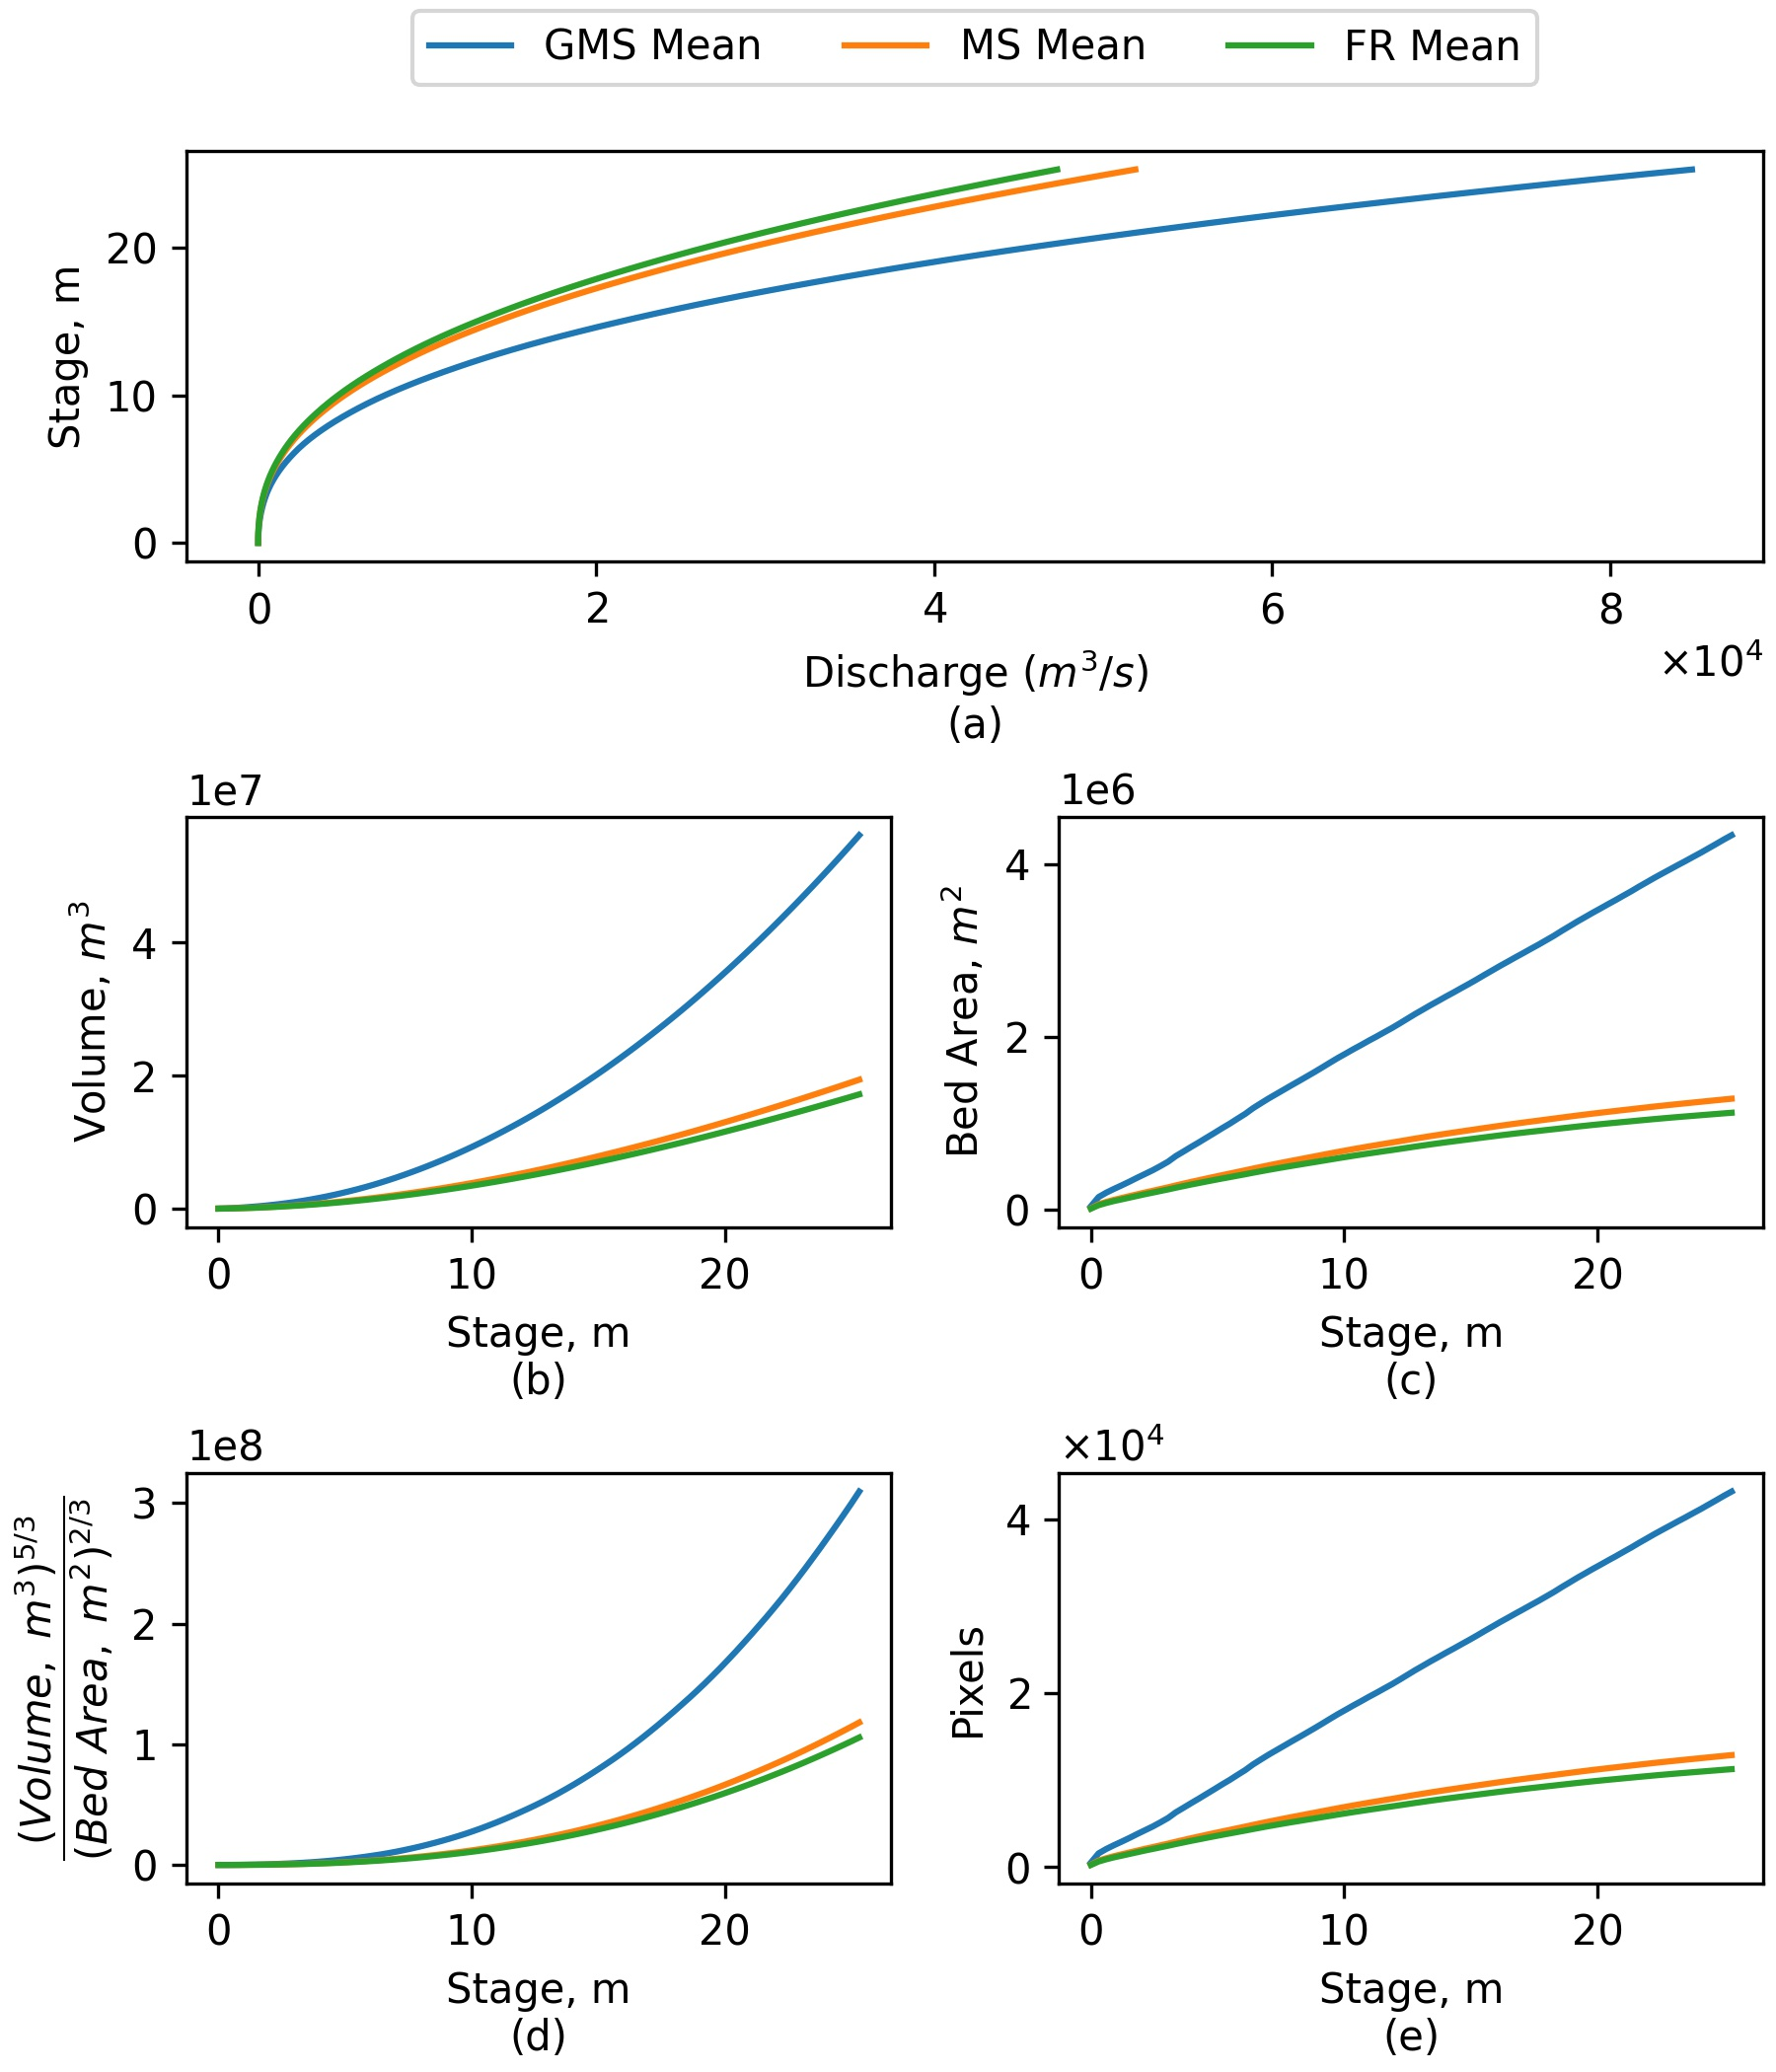
\includegraphics[scale=1.0]{figures/rating_curve_comparison.jpg}
    \caption{Illustrates average quantities for the three methods, FR, MS, and GMS, for each stage value (m). 
    The values are (a) Discharge $m^3s^{-1}$, (b) Volume $m^3$, (c) Bed Area $m^2$, (d) a function of Volume and Bed Area, and (e) number of pixels.
    }
    \label{fig:rating_curve_comparison}
    \end{figure}
    %
